\chapter{Topología en espacios finitos}\label{espaciosfinitos}
En esta sección vamos a hacer un breve resumen de las propiedades fundamentales de los espacios finitos que nos son de interés en el estudio de la forma. Las referencias fundamentales aqu'i son el libro \textit{Algebraic Topology of Finite Topological Spaces and Aplications} de J. A. Barmak \cite{barmak2011algebraic} y las notas publicadas por J. P. May \cite{jpmayfinitespaces}. 

La quintaesencia de la teoría de espacios finitos es que existe una correspondencia entre ellos y los conjuntos preordenados a través de los abiertos minimales: si para un punto $ x\in X  $ consideramos $ U_x  $ el abierto minimal que lo contiene, diremos que $ x\leq y  $ si $ U _{x } \subc U_y  $. Recíprocamente, podemos dotar a un conjunto preordenado de una topología dada por la base $ \{y\in X\mid y\leq x \}_{x\in X } $. Observamos además que los espacios $ T _{0 }  $ se corresponden con órdenes parciales y para los espacios finitos $ T_1  $ la topología es la discreta. 

Mediante esta asociaci'on, las aplicaciones continuas quedan caracterizadas como las que preservan el orden, y dos aplicaciones $f,g :X\lra Y $ son hom'otopas si existen otras aplicaciones $h_1,...,h_n$ que forman una cadena de desigualdades desde $f$ hasta $g$, por ejemplo $f\leq h_1\geq h_2\leq ... \leq h_n\geq g$.


La representación esquemática  más sencilla de un espacio finito es el llamado \textbf{diagrama de Hasse}: un grafo en el que cada punto de $X$ es un vértice y estos se unen según la relación de orden, de tal forma que empezamos desde los mayores y vamos trazando líneas hacia abajo hasta los menores.
\begin{example}
  Consideremos el espacio generado por la base 
  \begin{gather*}
      \{\{a\},\{b\},\{e\},\{c,e\},\{d,e\}\}.
  \end{gather*}
  Podemos representar su diagrama de Hasse como


\tikzset{every picture/.style={line width=0.75pt}} %set default line width to 0.75pt        
\begin{figure}[h]
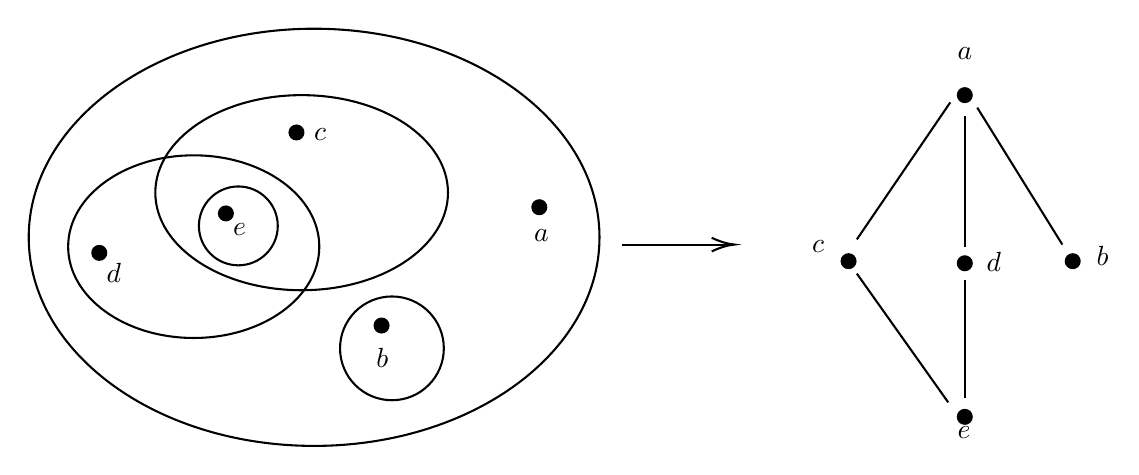
\begin{tikzpicture}[x=0.75pt,y=0.75pt,yscale=-1,xscale=1]
%uncomment if require: \path (0,310); %set diagram left start at 0, and has height of 310

%Shape: Ellipse [id:dp5345804384169703] 
\draw   (35,149.5) .. controls (35,94) and (96.56,49) .. (172.5,49) .. controls (248.44,49) and (310,94) .. (310,149.5) .. controls (310,205) and (248.44,250) .. (172.5,250) .. controls (96.56,250) and (35,205) .. (35,149.5) -- cycle ;
%Shape: Ellipse [id:dp3360173229986365] 
\draw   (54,154) .. controls (54,129.7) and (81.09,110) .. (114.5,110) .. controls (147.91,110) and (175,129.7) .. (175,154) .. controls (175,178.3) and (147.91,198) .. (114.5,198) .. controls (81.09,198) and (54,178.3) .. (54,154) -- cycle ;
%Shape: Ellipse [id:dp906562279151325] 
\draw   (96,128) .. controls (96,102.04) and (127.56,81) .. (166.5,81) .. controls (205.44,81) and (237,102.04) .. (237,128) .. controls (237,153.96) and (205.44,175) .. (166.5,175) .. controls (127.56,175) and (96,153.96) .. (96,128) -- cycle ;
%Shape: Circle [id:dp6114454362325152] 
\draw   (117,144) .. controls (117,133.51) and (125.51,125) .. (136,125) .. controls (146.49,125) and (155,133.51) .. (155,144) .. controls (155,154.49) and (146.49,163) .. (136,163) .. controls (125.51,163) and (117,154.49) .. (117,144) -- cycle ;
%Shape: Circle [id:dp27436024459221087] 
\draw   (185,203) .. controls (185,189.19) and (196.19,178) .. (210,178) .. controls (223.81,178) and (235,189.19) .. (235,203) .. controls (235,216.81) and (223.81,228) .. (210,228) .. controls (196.19,228) and (185,216.81) .. (185,203) -- cycle ;
%Straight Lines [id:da4272353897222474] 
\draw    (130,138) ;
\draw [shift={(130,138)}, rotate = 0] [color={rgb, 255:red, 0; green, 0; blue, 0 }  ][fill={rgb, 255:red, 0; green, 0; blue, 0 }  ][line width=0.75]      (0, 0) circle [x radius= 3.35, y radius= 3.35]   ;
%Straight Lines [id:da7898927205372115] 
\draw    (205,192) ;
\draw [shift={(205,192)}, rotate = 0] [color={rgb, 255:red, 0; green, 0; blue, 0 }  ][fill={rgb, 255:red, 0; green, 0; blue, 0 }  ][line width=0.75]      (0, 0) circle [x radius= 3.35, y radius= 3.35]   ;
%Straight Lines [id:da5195493562790454] 
\draw    (164,99) ;
\draw [shift={(164,99)}, rotate = 0] [color={rgb, 255:red, 0; green, 0; blue, 0 }  ][fill={rgb, 255:red, 0; green, 0; blue, 0 }  ][line width=0.75]      (0, 0) circle [x radius= 3.35, y radius= 3.35]   ;
%Straight Lines [id:da19253792016859794] 
\draw    (69,157) ;
\draw [shift={(69,157)}, rotate = 0] [color={rgb, 255:red, 0; green, 0; blue, 0 }  ][fill={rgb, 255:red, 0; green, 0; blue, 0 }  ][line width=0.75]      (0, 0) circle [x radius= 3.35, y radius= 3.35]   ;
%Straight Lines [id:da5961381889551676] 
\draw    (281,135) ;
\draw [shift={(281,135)}, rotate = 0] [color={rgb, 255:red, 0; green, 0; blue, 0 }  ][fill={rgb, 255:red, 0; green, 0; blue, 0 }  ][line width=0.75]      (0, 0) circle [x radius= 3.35, y radius= 3.35]   ;
%Straight Lines [id:da7815133080705046] 
\draw    (321,153) -- (373,153) ;
\draw [shift={(375,153)}, rotate = 180] [color={rgb, 255:red, 0; green, 0; blue, 0 }  ][line width=0.75]    (10.93,-3.29) .. controls (6.95,-1.4) and (3.31,-0.3) .. (0,0) .. controls (3.31,0.3) and (6.95,1.4) .. (10.93,3.29)   ;
%Straight Lines [id:da5410679949443915] 
\draw    (486,91) -- (486,154) ;
%Straight Lines [id:da4633778843673295] 
\draw    (486,81) ;
\draw [shift={(486,81)}, rotate = 0] [color={rgb, 255:red, 0; green, 0; blue, 0 }  ][fill={rgb, 255:red, 0; green, 0; blue, 0 }  ][line width=0.75]      (0, 0) circle [x radius= 3.35, y radius= 3.35]   ;
%Straight Lines [id:da5022133822677237] 
\draw    (486,162) ;
\draw [shift={(486,162)}, rotate = 0] [color={rgb, 255:red, 0; green, 0; blue, 0 }  ][fill={rgb, 255:red, 0; green, 0; blue, 0 }  ][line width=0.75]      (0, 0) circle [x radius= 3.35, y radius= 3.35]   ;
%Straight Lines [id:da3478985149182128] 
\draw    (486,170) -- (486,227) ;
%Straight Lines [id:da8148610978164064] 
\draw    (486,236) ;
\draw [shift={(486,236)}, rotate = 0] [color={rgb, 255:red, 0; green, 0; blue, 0 }  ][fill={rgb, 255:red, 0; green, 0; blue, 0 }  ][line width=0.75]      (0, 0) circle [x radius= 3.35, y radius= 3.35]   ;
%Straight Lines [id:da4544974333029552] 
\draw    (492,87) -- (533,153) ;
%Straight Lines [id:da6380421711344977] 
\draw    (538,161) ;
\draw [shift={(538,161)}, rotate = 0] [color={rgb, 255:red, 0; green, 0; blue, 0 }  ][fill={rgb, 255:red, 0; green, 0; blue, 0 }  ][line width=0.75]      (0, 0) circle [x radius= 3.35, y radius= 3.35]   ;
%Straight Lines [id:da39881988298363313] 
\draw    (434,167) -- (478,229) ;
%Straight Lines [id:da27751229522410403] 
\draw    (430,161) ;
\draw [shift={(430,161)}, rotate = 0] [color={rgb, 255:red, 0; green, 0; blue, 0 }  ][fill={rgb, 255:red, 0; green, 0; blue, 0 }  ][line width=0.75]      (0, 0) circle [x radius= 3.35, y radius= 3.35]   ;
%Straight Lines [id:da5728349321913497] 
\draw    (479,84.5) -- (434,150.5) ;

% Text Node
\draw (277,144.4) node [anchor=north west][inner sep=0.75pt]    {$a$};
% Text Node
\draw (201,201.4) node [anchor=north west][inner sep=0.75pt]    {$b$};
% Text Node
\draw (171,95.4) node [anchor=north west][inner sep=0.75pt]    {$c$};
% Text Node
\draw (71,160.4) node [anchor=north west][inner sep=0.75pt]    {$d$};
% Text Node
\draw (132,141.4) node [anchor=north west][inner sep=0.75pt]    {$e$};
% Text Node
\draw (481,56.4) node [anchor=north west][inner sep=0.75pt]    {$a$};
% Text Node
\draw (548,152.4) node [anchor=north west][inner sep=0.75pt]    {$b$};
% Text Node
\draw (481,239.4) node [anchor=north west][inner sep=0.75pt]    {$e$};
% Text Node
\draw (495,155.4) node [anchor=north west][inner sep=0.75pt]    {$d$};
% Text Node
\draw (411,149.4) node [anchor=north west][inner sep=0.75pt]    {$c$};


\end{tikzpicture}
\caption{Construcción del diagrama de Hasse a partir del espacio finito.}
\end{figure}
\end{example}


Esta representación nos ayuda, además, a reducir un espacio con retractos por deformación. Llamaremos a un punto \textbf{colapsable hacia abajo (arriba)} cuando en el diagrama de Hasse solo tenga una línea de salida (entrada). Estas condiciones son suficientes para asegurar que la aplicación que los envía hacia el punto inmediatemente inferior (superior) y fija el resto de puntos es un retracto por deformación. Si iteramos este proceso de reducci'on, llegamos a un espacio sin puntos colapsables, que llamaremos \textbf{espacio minimal}. Llamaremos \textbf{n'ucleo} de un espacio a su espacio minimal asociado. Esta ascociaci'on est'a bien definida por el siguiente teorema:

\begin{theorem}[Teorema de Clasificación]\label{clasif}
  Dos espacios finitos minimales homotópicamente equivalentes son homeomorfos. Asimismo, dos espacios finitos son homotópicamente equivalentes si y solo si sus núcleos son homeomorfos. En particular, todos los núcleos de un espacio son homeomorfos.
\end{theorem}




\section{Teoría de McCord}

La teor'ia de McCord, iniciada por 'el mismo en 1965 \cite{mccord}, relaciona los tipos de homotop'ia d'ebil de espacios finitos con los de complejos simpliciales finitos, demostrando que son exactamente los mismos.
                       
\begin{definition}
  Llamaremos \textbf{equivalencia homotópica débil} a una aplicación continua $ f:X\lra Y $ tal que $ f_{\dual} :\Pi_0(X,x_0)\lra \Pi_0(Y,f(x_0)) $ es biyectiva y 
  \begin{gather*}
    f_{\dual} :\Pi_n(X,x_0)\lra \Pi_n(Y,f(x_0))
  \end{gather*}
  es un isomorfismo para $ n\geq 1 $.
\end{definition}

Esta noción  no establece una relación de equivalencia entre espacios, puesto que no es simétrica.

Ahora, vamos a estudiar cómo asociar un complejo simplicial\footnote{Introducimos los conceptos fundamentales necesarios para el desarrollo de la teoría en el Apéndice \ref{apendice}.} a un espacio topológico de tal forma que se mantenga el tipo de homotopía débil:
\begin{definition}
  Dado un espacio $ X $ finito y $ T_0 $, el \textbf{complejo del orden} $ \kcal(X) $ es el que tiene por vértices los puntos de $X$ y por símplices a sus cadenas no vacías. Si $ f:X\lra Y $ es una función continua, se define la \textbf{función simplicial asociada} $ \kcal(f):\kcal(X)\lra \kcal(Y) $ por $ \kcal(f)(x)=f\px  $.
\end{definition}





\begin{theorem}
  Sea $ X $ un espacio topológico finito y $ T_0 $. La \textbf{aplicación de McCord} definida como 
  \begin{gather*}
    \begin{matrix}
    \mu_X: \ &\abs{\kcal(X)} &\longrightarrow &X \\
    &\alf  &\mapsto &\min \sop (\alf )
    \end{matrix}  
  \end{gather*}
  es una equivalencia homotópica débil.
\end{theorem}

\begin{observation}
  Dada una función continua $f$, el diagrama 
\begin{center}
\begin{tikzcd}
    \abs{\kcal(X)} \dar{\mu_X} \rar{\abs{\kcal(f)}} & \abs{\kcal(Y)} \dar{\mu_Y} \\ X \rar{f} & Y
\end{tikzcd}    
\end{center}
es conmutativo, y de hecho  \textbf{$f$ es equivalencia débil si y solo si $\kcal(f)$ es equivalencia homotópica}.
\end{observation}

Si partimos de un complejo simplicial, podemos obtener resultados homólogos mediante mediante el funtor $\xcal(\cdot)$, que asocia a cada complejo el conjunto parcialmente ordenado $\xcal(K)$ de símplices de $K$ ordenados por la inclusión. Este espacio se conoce como \textbf{espacio de caras} del complejo $K$. A las aplicaciones simpliciales $\vf:K\lra L $ les asocia aplicaciones continuas 
\begin{gather*}
    \begin{matrix*}
        \xcal(\vf):&\xcal(K)&\lra &\xcal(L) \\ 
        &\sigma &\mapsto & \vf(\sigma)
    \end{matrix*}
\end{gather*}

¿Qué complejo simplicial obtendremos al hacer $\kcal(\xcal(K))$? Los vértices serán los puntos de $\xcal(K)$, que son los símplices de $K$, y los símplices las cadenas de $\xcal(K)$, que son las cadenas de símplices de $K$. Esta es exactamente la descripción de la subdivisión baricéntrica de $K$ (ver \ref{subdiv}). Como existe un homeomorfismo $s_K$ entre $K'= \kcal(\xcal(K))   $ y $K$, definimos la aplicación de McCord
\begin{gather*}\label{apmccord2}
    \begin{matrix}
        \mu_K:&\abs{K}&\lra &\xcal(K) \\ 
        &\alf &\mapsto & \mu_K(\alf) = \mu_{\xcal(K)}\circ s_K\inv (\alf).
    \end{matrix}
\end{gather*}

Claramente, esta aplicación es una equivalencia homotópica débil, puesto que tanto $\mu_{\xcal(K)}$ como $s_K\inv $ lo son. Para aproximarnos a un resultado parecido al de la observación anterior, tenemos la siguiente

\begin{proposition}
  Dada una aplicación simplicial $\vf:K\lra L$ entre complejos, el siguiente diagrama conmuta en homotopía:
  \begin{center}
    \begin{tikzcd}
      \abs{K} \dar{\mu_K} \rar{\abs{\vf}} & \abs{L} \dar{\mu_L}\\ 
      \xcal(K) \rar{\xcal(\vf)} & \xcal(L)
  \end{tikzcd}
  \end{center}
\end{proposition}


\begin{corollary}
  Si $ \vf:K\lra L $ es una aplicación simplicial entre complejos finitos, entonces $ \abs{\vf } $ es una equivalencia homotópica si y solo si $ \xcal(\vf) $ es una equivalencia homotópica débil.
\end{corollary}




\begin{example}
  Analizamos el pseudocírculo. Sabemos que la aplicación de McCord es una equivalencia homotópica débil $\mu_{S^1}:\abs{\kcal(S^1)} = \mathbb{S}^1 \lra S^1 $. Sin embargo, no existe ninguna equivalencia débil en sentido contrario, puesto que cualquier función continua $ f:S^1\lra \mathbb{S}^1 $ es constante: como $ S^1 $ es conexo por caminos \cite{barmak2011algebraic} y $ f $ es continua, su imagen tiene que ser conexa por caminos. Al estar compuesta por $ 4 $ puntos en la circunferencia, estos tienen que coincidir, de tal forma que $ f $ es constante. Así, no puede existir tampoco una equivalencia homotópica entre ambos espacios. Como comentábamos en la introducción, esto constituye un contraejemplo del Teorema de Whitehead en espacios que no son CW-complejos.

\begin{figure}[h]
    \centering
    \tikzset{every picture/.style={line width=0.75pt}} %set default line width to 0.75pt        

\begin{tikzpicture}[x=0.75pt,y=0.75pt,yscale=-1,xscale=1]
%uncomment if require: \path (0,300); %set diagram left start at 0, and has height of 300

%Straight Lines [id:da9031632210185652] 
\draw    (91,108) ;
\draw [shift={(91,108)}, rotate = 0] [color={rgb, 255:red, 0; green, 0; blue, 0 }  ][fill={rgb, 255:red, 0; green, 0; blue, 0 }  ][line width=0.75]      (0, 0) circle [x radius= 3.35, y radius= 3.35]   ;
%Straight Lines [id:da7379643240071747] 
\draw    (91,191) ;
\draw [shift={(91,191)}, rotate = 0] [color={rgb, 255:red, 0; green, 0; blue, 0 }  ][fill={rgb, 255:red, 0; green, 0; blue, 0 }  ][line width=0.75]      (0, 0) circle [x radius= 3.35, y radius= 3.35]   ;
%Straight Lines [id:da8248239592746278] 
\draw    (170,109) ;
\draw [shift={(170,109)}, rotate = 0] [color={rgb, 255:red, 0; green, 0; blue, 0 }  ][fill={rgb, 255:red, 0; green, 0; blue, 0 }  ][line width=0.75]      (0, 0) circle [x radius= 3.35, y radius= 3.35]   ;
%Straight Lines [id:da25833856072266115] 
\draw    (170,192) ;
\draw [shift={(170,192)}, rotate = 0] [color={rgb, 255:red, 0; green, 0; blue, 0 }  ][fill={rgb, 255:red, 0; green, 0; blue, 0 }  ][line width=0.75]      (0, 0) circle [x radius= 3.35, y radius= 3.35]   ;
%Straight Lines [id:da4430343204757232] 
\draw    (90.8,114.8) -- (90.8,183.8) ;
%Straight Lines [id:da5180591167416297] 
\draw    (169.8,115.8) -- (169.8,184.8) ;
%Straight Lines [id:da167630388265398] 
\draw    (97,114) -- (163.8,187.8) ;
%Straight Lines [id:da23990421373738147] 
\draw    (162.8,112.8) -- (97.4,187.4) ;
%Curve Lines [id:da26154240547551977] 
\draw    (275,152) .. controls (314.6,122.3) and (334.6,180.81) .. (373.81,152.87) ;
\draw [shift={(375,152)}, rotate = 143.13] [color={rgb, 255:red, 0; green, 0; blue, 0 }  ][line width=0.75]    (10.93,-3.29) .. controls (6.95,-1.4) and (3.31,-0.3) .. (0,0) .. controls (3.31,0.3) and (6.95,1.4) .. (10.93,3.29)   ;
%Straight Lines [id:da8002884037042262] 
\draw    (518,109) ;
\draw [shift={(518,109)}, rotate = 0] [color={rgb, 255:red, 0; green, 0; blue, 0 }  ][fill={rgb, 255:red, 0; green, 0; blue, 0 }  ][line width=0.75]      (0, 0) circle [x radius= 3.35, y radius= 3.35]   ;
%Straight Lines [id:da8735860543705352] 
\draw    (443,152) ;
\draw [shift={(443,152)}, rotate = 0] [color={rgb, 255:red, 0; green, 0; blue, 0 }  ][fill={rgb, 255:red, 0; green, 0; blue, 0 }  ][line width=0.75]      (0, 0) circle [x radius= 3.35, y radius= 3.35]   ;
%Straight Lines [id:da4992437317056573] 
\draw    (599,152) ;
\draw [shift={(599,152)}, rotate = 0] [color={rgb, 255:red, 0; green, 0; blue, 0 }  ][fill={rgb, 255:red, 0; green, 0; blue, 0 }  ][line width=0.75]      (0, 0) circle [x radius= 3.35, y radius= 3.35]   ;
%Straight Lines [id:da2895031421856269] 
\draw    (521,194) ;
\draw [shift={(521,194)}, rotate = 0] [color={rgb, 255:red, 0; green, 0; blue, 0 }  ][fill={rgb, 255:red, 0; green, 0; blue, 0 }  ][line width=0.75]      (0, 0) circle [x radius= 3.35, y radius= 3.35]   ;
%Straight Lines [id:da9632575051202192] 
\draw    (518,109) -- (599,152) ;
%Straight Lines [id:da40384233245995205] 
\draw    (443,152) -- (521,194) ;
%Straight Lines [id:da8121868607433584] 
\draw    (521,194) -- (599,152) ;
%Straight Lines [id:da8423231776287685] 
\draw    (443,152) -- (518,109) ;

% Text Node
\draw (87,90.4) node [anchor=north west][inner sep=0.75pt]    {$a$};
% Text Node
\draw (166,88.4) node [anchor=north west][inner sep=0.75pt]    {$b$};
% Text Node
\draw (84,199.4) node [anchor=north west][inner sep=0.75pt]    {$c$};
% Text Node
\draw (165,197.4) node [anchor=north west][inner sep=0.75pt]    {$d$};
% Text Node
\draw (422,146.4) node [anchor=north west][inner sep=0.75pt]    {$a$};
% Text Node
\draw (606,142.4) node [anchor=north west][inner sep=0.75pt]    {$b$};
% Text Node
\draw (516,200.4) node [anchor=north west][inner sep=0.75pt]    {$c$};
% Text Node
\draw (513,85.4) node [anchor=north west][inner sep=0.75pt]    {$d$};
% Text Node
\draw (497,228.4) node [anchor=north west][inner sep=0.75pt]    {$\mathcal{K}\left( S^{1}\right)$};
% Text Node
\draw (120,232.4) node [anchor=north west][inner sep=0.75pt]    {$S^{1}$};


\end{tikzpicture}
    \caption{Complejo del orden del pseudocírculo $S^1$}
    \label{fig:my_label}
\end{figure}

Podemos calcular el espacio de caras de su compleo del orden, para obtener

\begin{figure}[h]
    \centering
\tikzset{every picture/.style={line width=0.75pt}} %set default line width to 0.75pt        

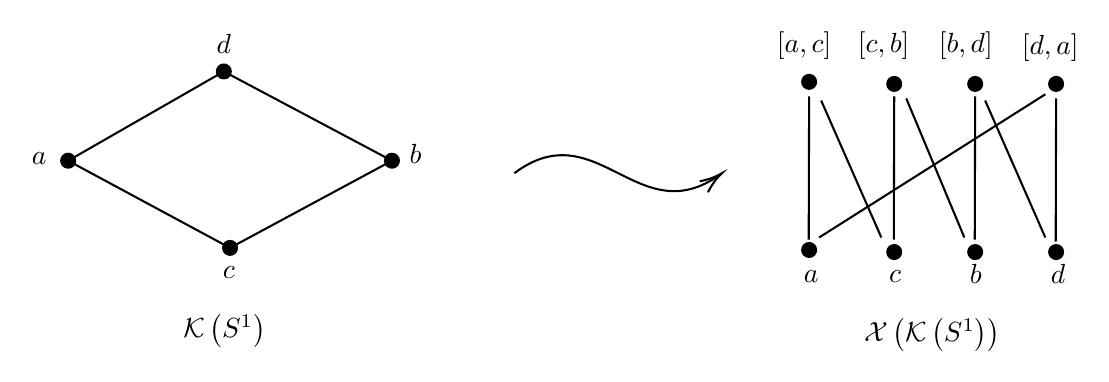
\begin{tikzpicture}[x=0.75pt,y=0.75pt,yscale=-1,xscale=1]
%uncomment if require: \path (0,300); %set diagram left start at 0, and has height of 300

%Straight Lines [id:da42313477533429267] 
\draw    (141,86) ;
\draw [shift={(141,86)}, rotate = 0] [color={rgb, 255:red, 0; green, 0; blue, 0 }  ][fill={rgb, 255:red, 0; green, 0; blue, 0 }  ][line width=0.75]      (0, 0) circle [x radius= 3.35, y radius= 3.35]   ;
%Straight Lines [id:da7938190023264293] 
\draw    (66,129) ;
\draw [shift={(66,129)}, rotate = 0] [color={rgb, 255:red, 0; green, 0; blue, 0 }  ][fill={rgb, 255:red, 0; green, 0; blue, 0 }  ][line width=0.75]      (0, 0) circle [x radius= 3.35, y radius= 3.35]   ;
%Straight Lines [id:da5956709678730521] 
\draw    (222,129) ;
\draw [shift={(222,129)}, rotate = 0] [color={rgb, 255:red, 0; green, 0; blue, 0 }  ][fill={rgb, 255:red, 0; green, 0; blue, 0 }  ][line width=0.75]      (0, 0) circle [x radius= 3.35, y radius= 3.35]   ;
%Straight Lines [id:da18839983802273164] 
\draw    (144,171) ;
\draw [shift={(144,171)}, rotate = 0] [color={rgb, 255:red, 0; green, 0; blue, 0 }  ][fill={rgb, 255:red, 0; green, 0; blue, 0 }  ][line width=0.75]      (0, 0) circle [x radius= 3.35, y radius= 3.35]   ;
%Straight Lines [id:da12882227112498512] 
\draw    (141,86) -- (222,129) ;
%Straight Lines [id:da9469846350495634] 
\draw    (66,129) -- (144,171) ;
%Straight Lines [id:da8066246644183905] 
\draw    (144,171) -- (222,129) ;
%Straight Lines [id:da7256277230658468] 
\draw    (66,129) -- (141,86) ;
%Curve Lines [id:da5721741782488827] 
\draw    (281,135) .. controls (320.6,105.3) and (340.6,163.81) .. (379.81,135.87) ;
\draw [shift={(381,135)}, rotate = 143.13] [color={rgb, 255:red, 0; green, 0; blue, 0 }  ][line width=0.75]    (10.93,-3.29) .. controls (6.95,-1.4) and (3.31,-0.3) .. (0,0) .. controls (3.31,0.3) and (6.95,1.4) .. (10.93,3.29)   ;
%Straight Lines [id:da06955161962394585] 
\draw    (423,91) ;
\draw [shift={(423,91)}, rotate = 0] [color={rgb, 255:red, 0; green, 0; blue, 0 }  ][fill={rgb, 255:red, 0; green, 0; blue, 0 }  ][line width=0.75]      (0, 0) circle [x radius= 3.35, y radius= 3.35]   ;
%Straight Lines [id:da6357974790134278] 
\draw    (464,92) ;
\draw [shift={(464,92)}, rotate = 0] [color={rgb, 255:red, 0; green, 0; blue, 0 }  ][fill={rgb, 255:red, 0; green, 0; blue, 0 }  ][line width=0.75]      (0, 0) circle [x radius= 3.35, y radius= 3.35]   ;
%Straight Lines [id:da7016506244526464] 
\draw    (503,92) ;
\draw [shift={(503,92)}, rotate = 0] [color={rgb, 255:red, 0; green, 0; blue, 0 }  ][fill={rgb, 255:red, 0; green, 0; blue, 0 }  ][line width=0.75]      (0, 0) circle [x radius= 3.35, y radius= 3.35]   ;
%Straight Lines [id:da8356774423464148] 
\draw    (542,92) ;
\draw [shift={(542,92)}, rotate = 0] [color={rgb, 255:red, 0; green, 0; blue, 0 }  ][fill={rgb, 255:red, 0; green, 0; blue, 0 }  ][line width=0.75]      (0, 0) circle [x radius= 3.35, y radius= 3.35]   ;
%Straight Lines [id:da42510834464203295] 
\draw    (423,172) ;
\draw [shift={(423,172)}, rotate = 0] [color={rgb, 255:red, 0; green, 0; blue, 0 }  ][fill={rgb, 255:red, 0; green, 0; blue, 0 }  ][line width=0.75]      (0, 0) circle [x radius= 3.35, y radius= 3.35]   ;
%Straight Lines [id:da3008866374740782] 
\draw    (464,173) ;
\draw [shift={(464,173)}, rotate = 0] [color={rgb, 255:red, 0; green, 0; blue, 0 }  ][fill={rgb, 255:red, 0; green, 0; blue, 0 }  ][line width=0.75]      (0, 0) circle [x radius= 3.35, y radius= 3.35]   ;
%Straight Lines [id:da9886139467140811] 
\draw    (503,173) ;
\draw [shift={(503,173)}, rotate = 0] [color={rgb, 255:red, 0; green, 0; blue, 0 }  ][fill={rgb, 255:red, 0; green, 0; blue, 0 }  ][line width=0.75]      (0, 0) circle [x radius= 3.35, y radius= 3.35]   ;
%Straight Lines [id:da16581959760579412] 
\draw    (542,173) ;
\draw [shift={(542,173)}, rotate = 0] [color={rgb, 255:red, 0; green, 0; blue, 0 }  ][fill={rgb, 255:red, 0; green, 0; blue, 0 }  ][line width=0.75]      (0, 0) circle [x radius= 3.35, y radius= 3.35]   ;
%Straight Lines [id:da7796706954720523] 
\draw    (423,98) -- (422.8,167) ;
%Straight Lines [id:da9140322482688465] 
\draw    (464,98) -- (463.8,167) ;
%Straight Lines [id:da2104472141788425] 
\draw    (503,98) -- (502.8,167) ;
%Straight Lines [id:da44498134430033676] 
\draw    (542,99) -- (541.8,168) ;
%Straight Lines [id:da20057634970027127] 
\draw    (428.8,100) -- (457.8,166) ;
%Straight Lines [id:da018454376193318245] 
\draw    (469.8,99) -- (497.8,166) ;
%Straight Lines [id:da6454286644172489] 
\draw    (507.8,100) -- (536.8,166) ;
%Straight Lines [id:da252545358736624] 
\draw    (536.8,97) -- (427.8,166) ;

% Text Node
\draw (47,123.4) node [anchor=north west][inner sep=0.75pt]    {$a$};
% Text Node
\draw (229,119.4) node [anchor=north west][inner sep=0.75pt]    {$b$};
% Text Node
\draw (139,178.4) node [anchor=north west][inner sep=0.75pt]    {$c$};
% Text Node
\draw (136,66.4) node [anchor=north west][inner sep=0.75pt]    {$d$};
% Text Node
\draw (120,201.4) node [anchor=north west][inner sep=0.75pt]    {$\mathcal{K}\left( S^{1}\right)$};
% Text Node
\draw (406,65.4) node [anchor=north west][inner sep=0.75pt]    {$[ a,c]$};
% Text Node
\draw (445,65.4) node [anchor=north west][inner sep=0.75pt]    {$[ c,b]$};
% Text Node
\draw (484,65.4) node [anchor=north west][inner sep=0.75pt]    {$[ b,d]$};
% Text Node
\draw (524,66.4) node [anchor=north west][inner sep=0.75pt]    {$[ d,a]$};
% Text Node
\draw (419,180.4) node [anchor=north west][inner sep=0.75pt]    {$a$};
% Text Node
\draw (460,180.4) node [anchor=north west][inner sep=0.75pt]    {$c$};
% Text Node
\draw (499,177.4) node [anchor=north west][inner sep=0.75pt]    {$b$};
% Text Node
\draw (538,177.4) node [anchor=north west][inner sep=0.75pt]    {$d$};
% Text Node
\draw (448,203.4) node [anchor=north west][inner sep=0.75pt]    {$\mathcal{X}\left(\mathcal{K}\left( S^{1}\right)\right)$};


\end{tikzpicture}
    \caption{Espacio de caras del complejo $\kcal(S^1)$.}
    \label{fig:my_label2}
\end{figure}
\end{example}